\chapter{Natural Language Processing}

\begin{itemize}
\item 
Solve sequence transduction, i.e., transforms an input sequence to an output sequence.

\item 
Necessary to have some \textit{memory}.
\end{itemize}

\section{RNN}
\begin{itemize}
\item 
At each time step, receive two inputs: word embedding of current word and hidden state.

\item 
Let $x_t \in \R^{n}$ and $h_{t-1} \in \R^{m}.$

\item 
Use weight matrix $W_{x} \in \R^{m \times n}$ and hidden-state-to-hidden-state matrix $W_{h} \in \R^{m\times m}.$

\item 
Then 
\begin{align*}
	o_t &= W_{hh} h_{t-1} + W_{hx} x_t + b_h\\
	h_t &= \tanh(o_t) = \tanh(W_h \cdot [h_{t-1}, x_t] + b_h)\\
	y_t &= g(W_y h_t + b_y)
\end{align*}
for some activation function $g.$

\item 
We can show that 
\[ \nabla_{W_{hh}}(h_t) = \sum_{t^\prime = 1}^{t-1} h_{t^\prime} \left( W_{hh}^{t-t^\prime-1} \tanh'(o_{t^\prime+1}) \cdot \cdots \cdot  \tanh^\prime(o_{t}) \right). \]
So the influence of $h_{t'}$ on $h_{t}$ will be small if $t' \ll t$ as $\tanh(x)$ is small for $|x| > 2,$ i.e., we have a \textit{vanishing gradient problem}.

\end{itemize}

\section{LSTM}

\begin{itemize}
\item 
Introduce \textit{cell state} to RNN.

\item
Information is added or removed to the cell state through \textit{gates}.

\item 
\textbf{Forget gate}:
	\begin{itemize}
	\item Input: previous cell state $C_{t-1}$ and $x_t.$
	\item Output: number in $[0,1]$ for each entry in $C_{t-1},$ i.e., how much to forget.
	\item So we have
		\begin{align*}
		f_t &=  \sigma(W_{hf}h_{t-1} + W_{xf}x_t + b_f)\\
		    &=\sigma ( W_f \cdot [h_{t-1}, x_t] + b_f),
		\end{align*}
	where $\sigma$ is the sigmoid function applied element-wise.
	\end{itemize}

\item 
\textbf{Input and update gate}:
	\begin{itemize}
	\item 
	Decide what and how much to add to the cell state.
	
	\item 
	What to add: \[ \tilde{C}_t = \tanh(W_C \cdot [h_{t-1}, x_t] + b_C). \]
	
	\item 
	How much to add: \[ i_t = \sigma(W_i \cdot [h_{t-1}, x_t] + b_i). \]
	
	\item 
	Update cell state: \[ C_t = f_t \odot C_{t-1} + i_t \odot \tilde{C}_t, \] where $\odot$ is element-wise multiplication.
	\end{itemize}

\item 
\textbf{Output gate}:
	\begin{itemize}
	\item 
	Decide what parts of cell state to output: \[ o_t = \sigma(W_o \cdot [h_{t-1}, x_t] + b_o). \]
	
	\item 
	Actual output: \[ h_t = o_t \odot \tanh(C_t) \]
	\end{itemize}

\item 
Drawbacks: computational complexity, overfitting, dropout harder to implement, sensitive to different random weight initializations, inability to handle temporal dependencies that are longer than a few steps, 

\end{itemize}

\section{Seq2seq}

\begin{itemize}
\item 
Input \textrightarrow{} Encoder \textrightarrow{} Context Vector \textrightarrow{} Decoder \textrightarrow{} Output

\item 
Encoder and decoder are both RNNs or LSTMs.

\item 
Last hidden state of encoder is context vector, which initializes decoder RNN.

\item 
At each time step, decoder receives previous token (input of RNN) and uses previous hidden state. The output of RNN is fed though FNN to get embedding of word.

\item 
Stop when EOS token is outputted.

\item 
For back-propagation, \textit{teacher forcing} is used, i.e., plug in correct words to decoder and stop at correct length.

\item Drawbacks:
\begin{itemize}
\item 
Bottleneck problem: for long input sequences, information would tend to be lost.

\item 
For the decoder, different information may be relevant at different steps.
\end{itemize}
\begin{figure}[ht]
	\centering
	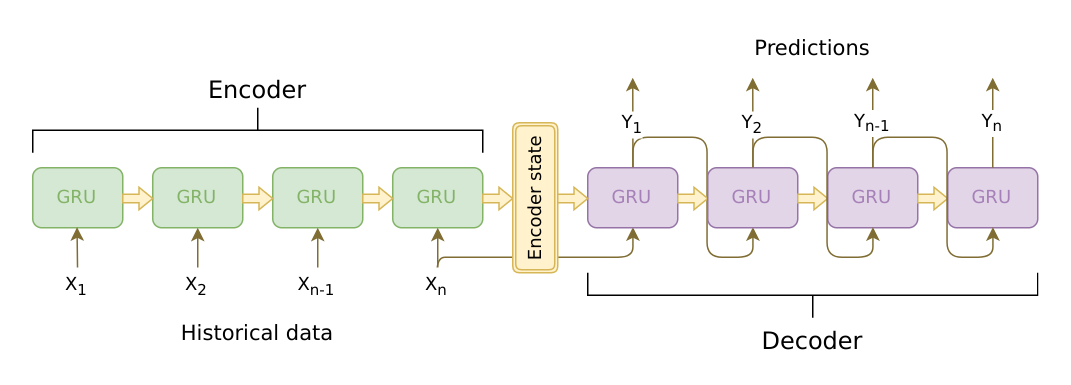
\includegraphics[width=\textwidth]{seq2seq}
	\caption*{Image source: \cite{seq2seq_eddy}}
\end{figure}
\end{itemize}

\section{Seq2seq with Attention}

\begin{itemize}
\item 
At each decoder step, it decides which source parts are more important

\item Concretely, at each $t,$:
	\begin{enumerate}[label=(\roman*)]
	\item
	Use previous token in RNN to update hidden state $h_t.$
	
	\item 
	Compute  $\score(h_t,s_k)$ between decoder hidden state $h_t$ and all encoder hidden states $s_1,\ldots,s_m;$
	
	\item 
	Compute attention weights: softmax attention scores;
	
	\item 
	Compute attention vector $a_t$: weighted sum of encoder states.
	
	\item 
	Use attention vector $a_t$ and hidden state $h_t$ in FNN to get output token.
	\end{enumerate}

\item Popular score functions:
	\begin{itemize}
	\item 
	Dot-product: $\score(h_t,s_k) = h_t^T s_k.$
	
	\item 
	Bilinear function: $\score(h_t,s_k) = h_t^T W s_k.$
	
	\item 
	Multi-layer perceptron: $\score(h_t,s_k) = v^T\tanh(W[h_t,s_k]).$
	\end{itemize}

\item Drawback: RNN is difficult to parallelize.

\begin{figure}[ht]
	\centering
	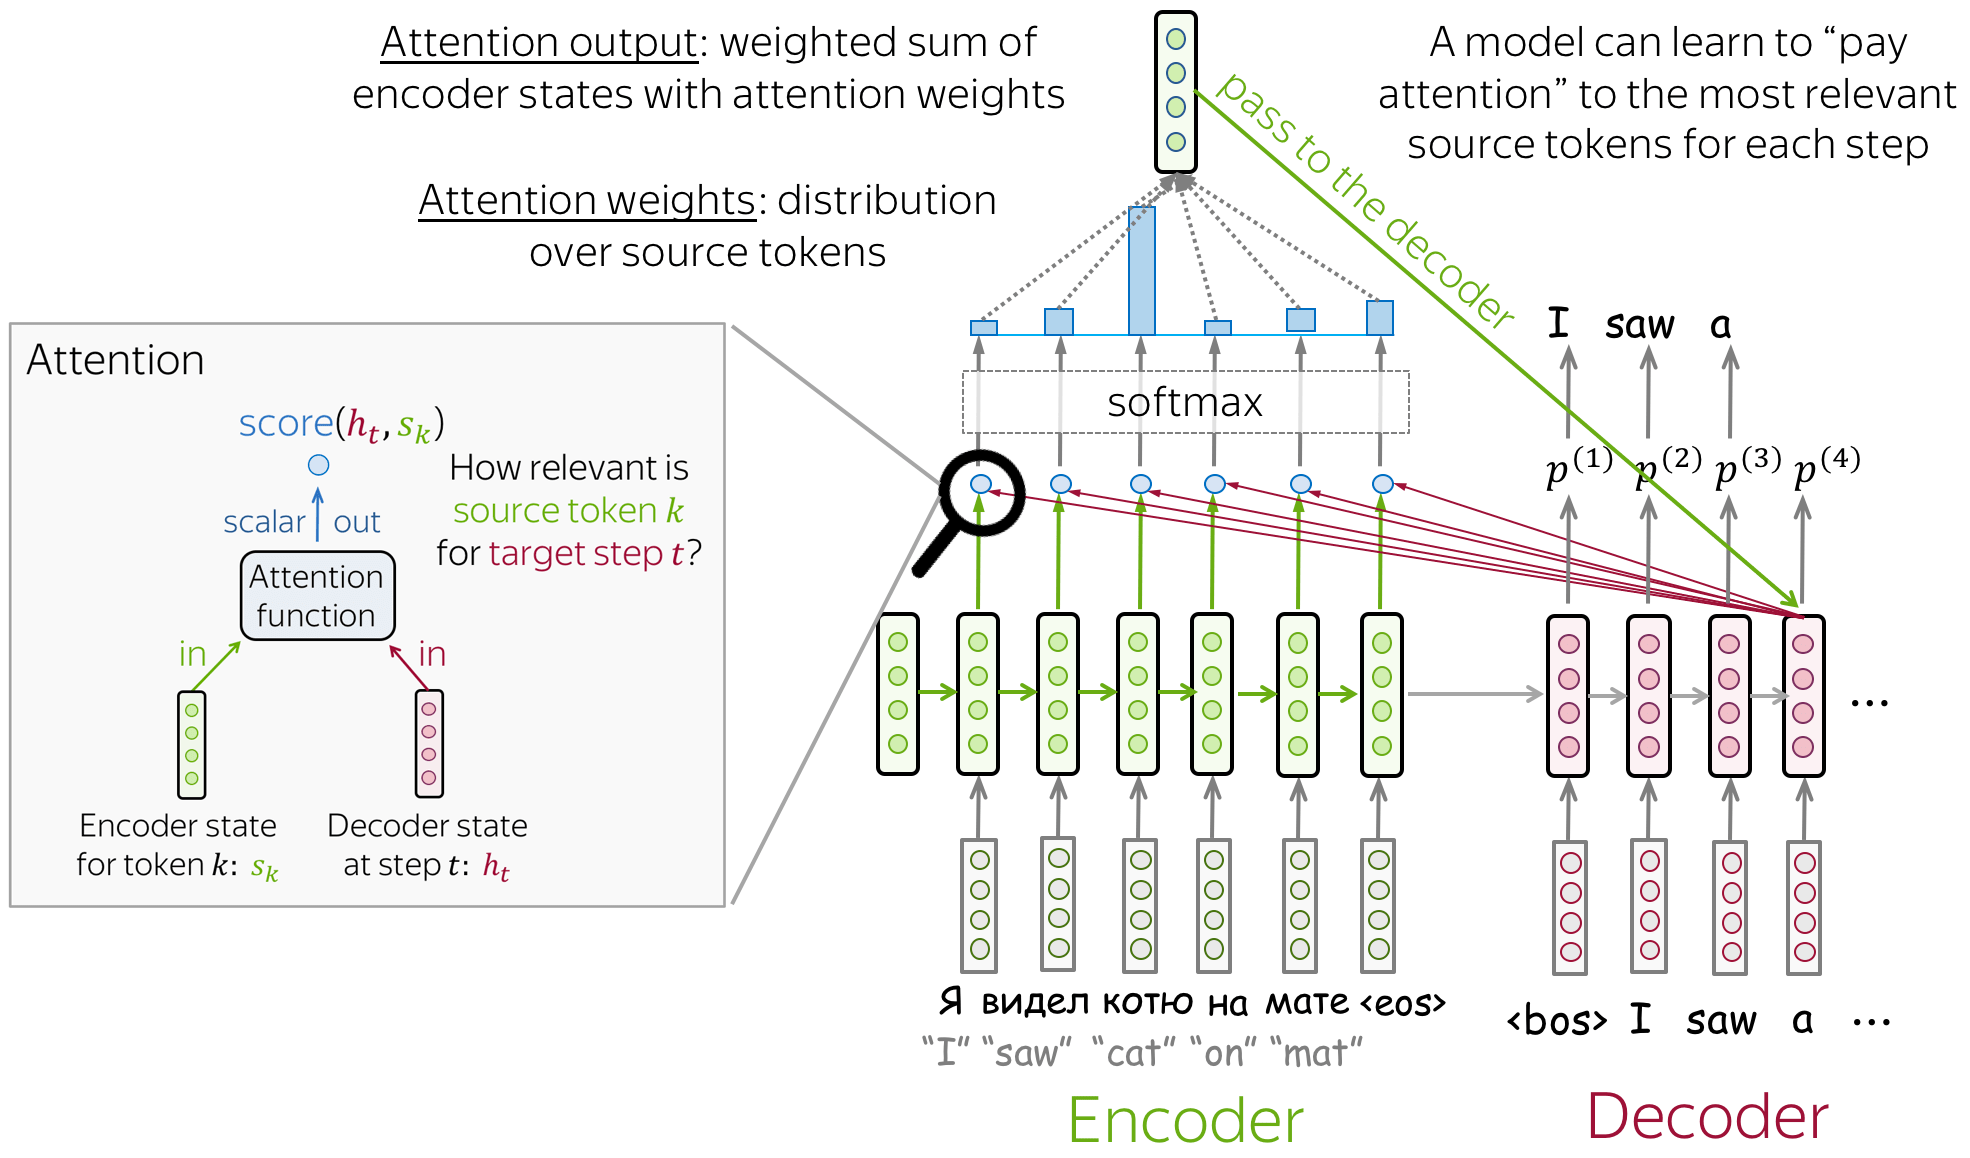
\includegraphics[width=\textwidth]{seq2seq_attention}
	\caption*{Image source: \cite{seq2seq_voita}}
\end{figure}
\end{itemize}